\documentclass[a4paper,12pt]{article}
\usepackage[left=1.8cm,right=1.8cm,top=2.5cm,bottom=2.5cm]{geometry} % Adjust page margins
\usepackage{xcolor,graphicx,framed}
\usepackage[normalem]{ulem}
\usepackage{amsmath}
\usepackage{cases}
\usepackage{gensymb}
\usepackage{chemmacros}
\setlength{\extrarowheight}{0.4cm}

\begin{document}

\newcommand{\HRule}{\rule{\linewidth}{0.4mm}} % Defines a new command for the horizontal lines, change thickness here

%----------------------------------------------------------------------------------------
%	HEADING SECTIONS
%----------------------------------------------------------------------------------------

\begin{minipage}{0.7\textwidth}
\begin{flushleft} 
\textsc{Universidad del Valle de Guatemala \\
Campus Central \\
Facultad de Ciencias y Humanidades \\
Departamento de Qu\'imica \\
Segundo ciclo, 2014 \\
Fisicoqu\'imica 1 \\
Secci\'on 10 \\
}
\end{flushleft}
\end{minipage}
~
\begin{minipage}{0.2\textwidth}
\begin{flushright}

\includegraphics[scale=0.35]{Logo_UVG} % Include a department/university logo
\end{flushright}
\end{minipage}\\

%----------------------------------------------------------------------------------------
%	TITLE SECTION
%----------------------------------------------------------------------------------------

\begin{center}
\HRule \\[0.4cm]
{ \bfseries Evaluaci\'on 4}\\ % Title of your document
\HRule \\[0.4cm]
\end{center}

%----------------------------------------------------------------------------------------

\section*{Instrucciones}

Responder y resolver los siguientes problemas en las hojas adicionales haciendo uso de regla, calculadora cient\'ifica, una tabla peri\'odica y el formulario individual que haya sido previamente aprobado para su uso. Cualquier actitud deshonesta ser\'a sancionada seg\'un el C\'odigo de comportamiento de los estudiantes de la Universidad.

\section*{Problemas}

\begin{enumerate}

 \item (10 pts) Indicar para cada uno de los siguientes enunciados si es verdadero o falso: % Problema F/V (10 preguntas)
\begin{enumerate}
 \item En una soluci\'on ideal no aplica la ley de Henry para el soluto.
 \item Una desviaci\'on positiva de la ley de Raoult produce una mezcla azeotr\'opica de punto de ebullici\'on m\'aximo.
 \item Aumentar la temperatura para una reacci\'on exot\'ermica que est\'a en equilibrio favorece a los reactivos.
 \item Si una reacci\'on qu\'imica est\'a en equilibrio, se tiene que $K=0$.
 \item Las propiedades molares parciales son propiedades extensivas.
\end{enumerate}

 \item (15 pts) Una mezcla de etanol y \emph{n}-propanol se comporta de manera ideal a $36.4\,\celsius$; a esa temperatura las presiones de vapor en equilibrio del etanol y \emph{n}-propanol son $108\;\mbox{mmHg}$ y $40.0\;\mbox{mmHg}$, respectivamente. Dibujar el diagrama de fase de presi\'on de vapor de este sistema a $36.4\,\celsius$ (para la parte de vapor, pueden evaluar por lo menos tres puntos de la presi\'on total para darse una idea de c\'omo es el l\'imite de fase). % Problema de hacer un diagrama de presion-composicion: datos del problema 7.26 de Chang.

 \item (15 pts) El etilenglicol $\mbox{CH}_2\mbox{(OH)CH}_2\mbox{(OH)}$ es un anticongelante com\'un para radiadores de autom\'oviles. ?`Cu\'antos mililitros de esta sustancia agregar\'ia a $6.5\;\mbox{L}$ de agua en el radiador de un carro en New York si el d\'ia m\'as fr\'io en el invierno es de $-20\,\celsius$? ?`Mantendr\'ia esta sustancia en el radiador durante el verano para evitar que hierva el agua? (La densidad y el punto de ebullici\'on del etilenglicol son $1.11\;\mbox{g}\cdot\mbox{cm}^{-3}$ y $470\;\mbox{K}$, respectivamente. La densidad y $K_f$ para el agua son $1.00\;\mbox{g}\cdot\mbox{cm}^{-3}$ y $1.86\;\mbox{K}\cdot\mbox{kg}\cdot\mbox{mol}^{-1}$, respectivamente.) % Problema de propiedades coligativas: problema 7.33 de Chang.

 \item (20 pts) La energ\'ia de Gibbs est\'andar de formaci\'on del $\mbox{NH}_3\mbox{(g)}$ es $-16.5\;\mbox{kJ}\cdot\mbox{mol}^{-1}$ a $298\;\mbox{K}$. ?`Cu\'al es la energ\'ia de Gibbs de reacci\'on cuando las presiones parciales respectivas del $\mbox{N}_2$, $\mbox{H}_2$ y $\mbox{NH}_3$ (tratados como gases ideales) son $3.0\;\mbox{bar}$, $1.0\;\mbox{bar}$ y $4.0\;\mbox{bar}$? ?`Cu\'al es la direcci\'on de la reacci\'on espont\'anea a partir de ese punto? % Problema de equilibrio quimico: 6.17(a) de Atkins.

 \item (15 pts) Considere la siguiente reacci\'on:
$$\mbox{CO}_2\mbox{(g)}+\mbox{H}_2\mbox{(g)}\;\ch{ <=> }\;\mbox{CO(g)}+\mbox{H}_2\mbox{O(g)}$$
La constante de equilibrio es de $0.534$ a $960\;\mbox{K}$ y de $1.571$ a $1\,260\;\mbox{K}$. Calcular el cambio de entalp\'ia y el cambio de entrop\'ia de la reacci\'on. % Problema de ecuacion de van 't Hoff: problema 9.9 de Chang.

 \item (25 pts) La siguiente figura muestra los diagramas de fase determinados experimentalmente para la soluci\'on casi ideal entre el hexano y el heptano.
\begin{enumerate}
 \item Indicar en cada regi\'on de los diagramas las fases que est\'an presentes.
 \item Para una soluci\'on que contiene $1\;\mbox{mol}$ de cada uno de los componentes, estimar la presi\'on de vapor a $70\,\celsius$ cuando la vaporizaci\'on comienza por reducci\'on de la presi\'on externa.
 \item ?`Cu\'al es la presi\'on de vapor de la soluci\'on a $70\,\celsius$ cuando queda s\'olo una gota del l\'iquido?
 \item Estimar con las figuras la fracci\'on molar del hexano en las fases l\'iquida y vapor en las condiciones del segundo inciso.
 \item ?`Cu\'ales son las fracciones molares para las condiciones del tercer inciso?
 \item A $85\,\celsius$ y $760\;\mbox{Torr}$, ?`cu\'ales son las cantidades de sustancia en cada fase cuando $z_{heptano}=0.40$?
\end{enumerate}

\begin{center}
 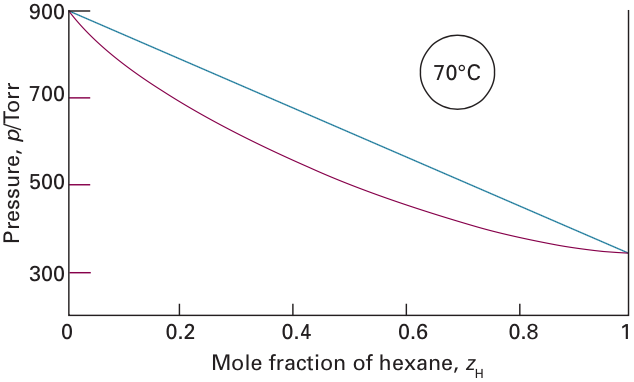
\includegraphics[scale=0.46]{figure2}
\end{center}

\begin{center}
 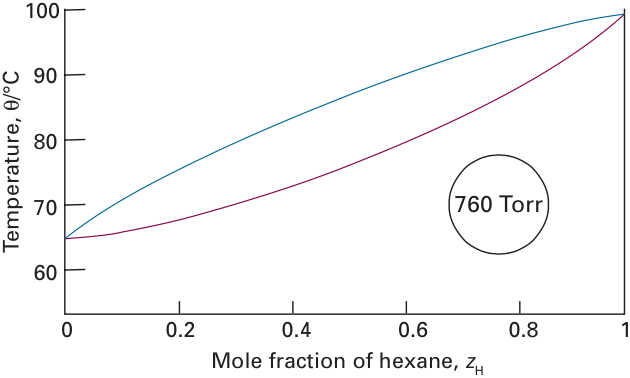
\includegraphics[scale=0.46]{figure3}
\end{center} % Problema de interpretar un diagrama de temperatura-composicion: 5.32(a) de Atkins.

\end{enumerate}

\end{document}
